\documentclass[aspectratio=169]{beamer}
\usetheme{Madrid}
\usepackage[utf8]{inputenc}
\usepackage[T1]{fontenc}
\usepackage{tikz}
\usepackage{amssymb}
\usepackage{graphicx}
\setbeamertemplate{navigation symbols}{}
\setbeamercolor{title}{fg=white,bg=orange!85!red}
\setbeamercolor{frametitle}{fg=white,bg=orange!85!red}
\setbeamercolor{block title}{bg=orange!85!red!20,fg=black}
\setbeamercolor{block body}{bg=orange!85!red!8,fg=black}
\setbeamercolor{item}{fg=orange!85!red}
\setbeamercolor{itemize item}{fg=orange!85!red}
\setbeamertemplate{itemize item}[triangle]

\title{Block Arcade 2 — Motion \& Repeat}
\subtitle{"Repeat" blocks — do something several times without copy-pasting}
\author{ByteForge --- Grade 7 --- Game Maker}
\date{}

\begin{document}

\begin{frame}
    \titlepage
\end{frame}

\begin{frame}{Today's Plan}
    \begin{itemize}
        \item Repeat 3 Times
        \item Marching Line
        \item[$\bigstar$] BOSS --- Bouncing Sprite
    \end{itemize}
\end{frame}

\begin{frame}{Repeat — do it without repeating yourself}
    \large
    \begin{itemize}
        \item "Repeat 3" scales
        \item Drawing 30 sprites by hand would mean 30 blocks, while a repeat block handles any number.
    \end{itemize}

    \begin{center}
    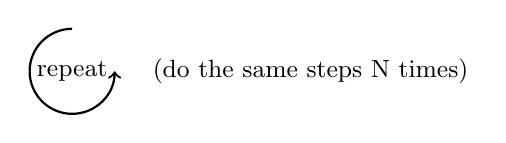
\begin{tikzpicture}[scale=0.9]

        \draw[->, thick] (0,0) arc (90:360:0.6);
        \node at (0,-0.6) {\small repeat};
        \node[right] at (1,-0.6) {\small (do the same steps N times)};
    \end{tikzpicture}
    \end{center}
\end{frame}


\begin{frame}{A variable changing INSIDE a loop}
    \large
    \begin{itemize}
        \item Changing x by 80 each pass through the loop is what actually spaces the sprites out.
        \item Worked example: repeat 5 times, changing x by 80 each pass, starting at x=20, places sprites at x = 20, 100, 180, 260, 340 — five different positions from ONE block stacked once.
    \end{itemize}
\end{frame}


\begin{frame}{BOSS — movement is a variable changing every frame}
    \large
    \begin{itemize}
        \item "On every frame" is a repeat block that never stops. That's genuinely what ALL motion in ALL games actually is.
    \end{itemize}
\end{frame}

\begin{frame}{Real-World Examples}
    \large
    \begin{itemize}
        \item A marching band or a row of parked cars, evenly spaced
        \item The spacing pattern (each one a fixed distance from the last) is the exact "loop + changing variable" idea. Minecraft building a straight fence or a row of torches is the same repeat pattern, just done by hand instead of by a loop.
    \end{itemize}
\end{frame}


\begin{frame}{Image}
    \begin{center}
    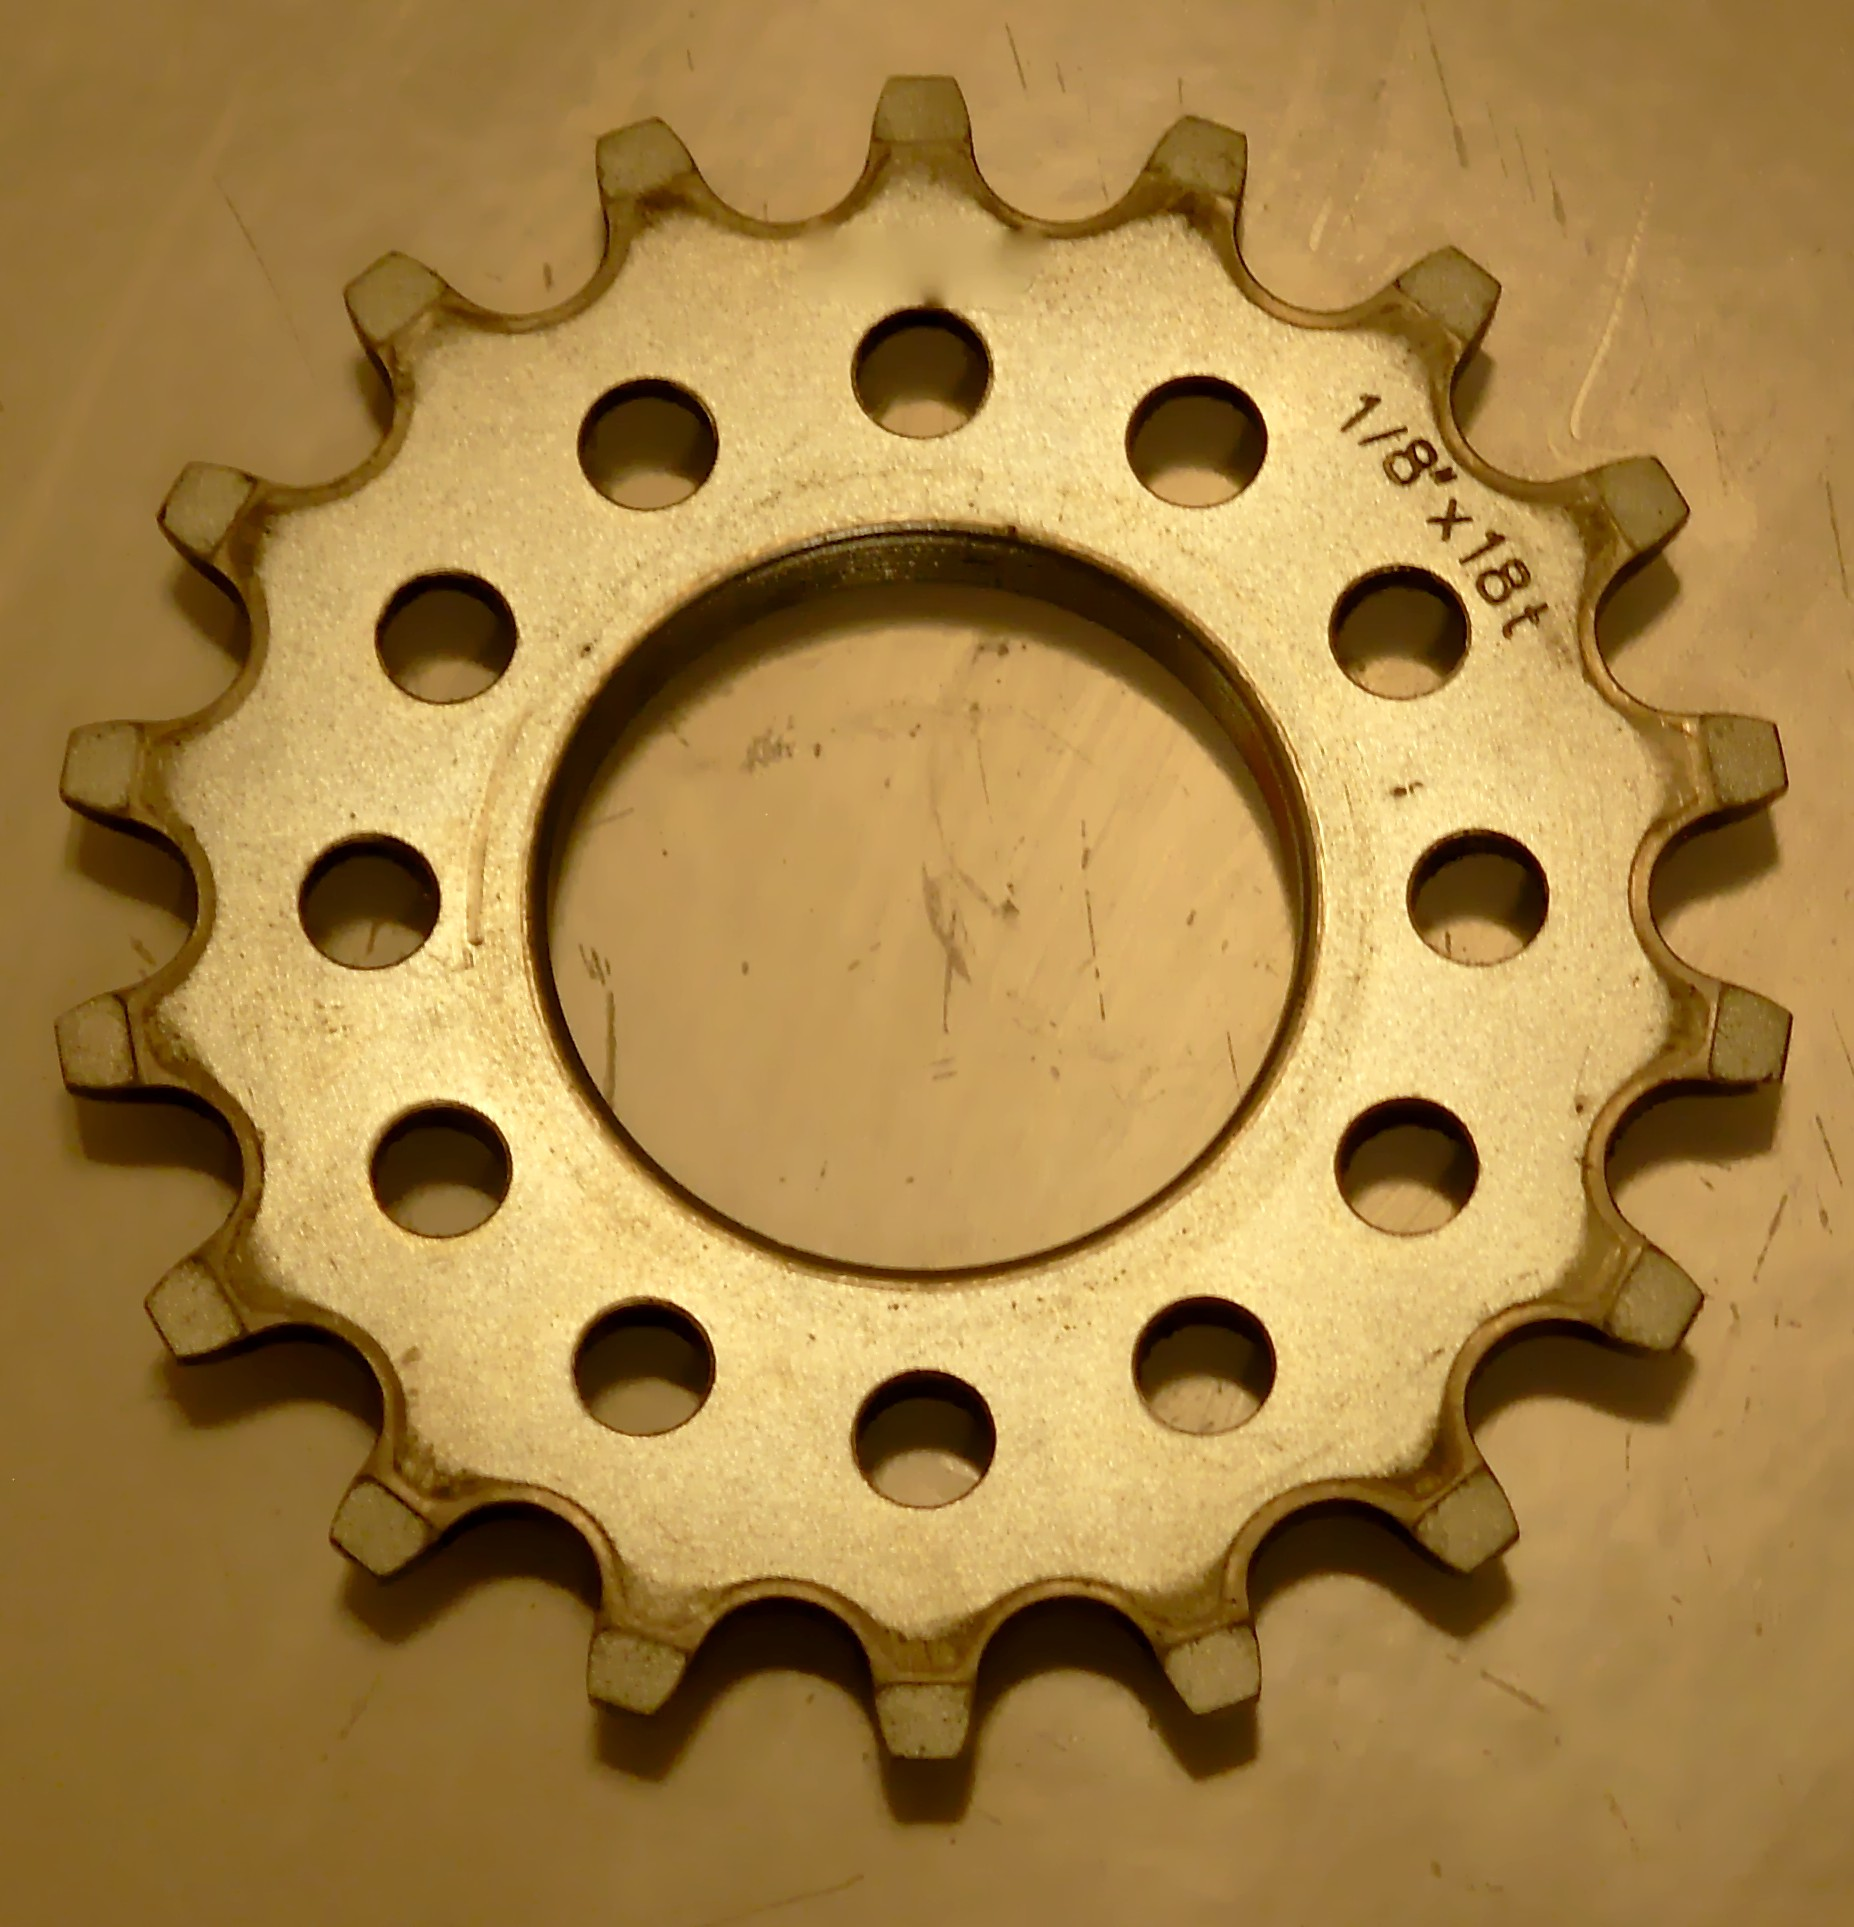
\includegraphics[width=0.5\textwidth]{images/gear.jpg}

    \large A gear does the same defined turn every time it's driven --- like a loop repeating the same steps.

    \small Fixed gear cog — John Reaves, public domain, via Wikimedia Commons
    \end{center}
\end{frame}

\begin{frame}{Let Them Discover}
    \Large
    Watch any 2D platformer character walk for 10 seconds. Roughly how many times does it "step" a tiny bit? Movement that looks smooth is secretly hundreds of small repeats — try to spot the individual frames.
\end{frame}

\begin{frame}{Your Turn}
    \Large
    Open the student map, find \textbf{Block Arcade 2 — Motion \& Repeat}, and work through it
    hands-on --- everything you just saw, they now do themselves.
\end{frame}

\end{document}
